\documentclass[a4paper]{article}

% Pacotes para o português.
\usepackage[brazilian]{babel}
\usepackage[utf8]{inputenc}
\usepackage[T1]{fontenc}

\usepackage{datetime}
\usepackage{graphicx}

% Usado nos pedaços de código.
\usepackage{listings}
\lstset{language=C,
	basicstyle=\small\sffamily,
	numbers=left,
	numberstyle=\tiny,
	frame=tb,
	columns=fullflexible,
	showstringspaces=false,
	captionpos=b}
\renewcommand\lstlistingname{Código}

\newcommand{\HRule}{\rule{\linewidth}{0.5mm}}

\begin{document}

\begin{titlepage}
\begin{center}	

% Topo 1.
\textsc{\Large UNIVERSIDADE DE SÃO PAULO\\
	INSTITUTO DE CIÊNCIAS MATEMÁTICAS E DE COMPUTAÇÃO}\\[0.7cm]

% Topo 2.
\textsc{\Large SSC0143}\\[0.2cm]
\textsc{\Large Programação Concorrente - Turma B}\\[0.5cm]

% Título.
\HRule \\[0.4cm]
{ \huge \bfseries Palíndromos}\\[0.4cm]
\HRule \\[0.4cm]
\textsc{Professor Dr. Julio Estrella}\\[1.5cm]

% Grupo
\begin{minipage}{0.4\textwidth}
\begin{flushleft} \large
\emph{Grupo 06:}\\
Bruno Junqueira Adami\\
Lucas Junqueira Adami\\
Lucas Lobosque\\
\end{flushleft}
\end{minipage}
\begin{minipage}{0.4\textwidth}
\begin{flushright} \large
\emph{Números USP:}\\
6878762\\
6792496\\
6792645\\
\end{flushright}
\end{minipage}

\vfill

% Rodapé.
{\large \today}
	
\end{center}
\end{titlepage}

\section{Introdução}
\indent \indent O problema proposto é o de devesenvolver versões de um programa paralelo para realizar as tarefas de determinar a ocorrência de palíndromos em dois textos especificados. Além disso, no texto maior, uma vez encontrado o palíndromo, é preciso determinar se a soma dos números correspondentes ao mapeamento do código ASCII de cada caracter da palavra é um número primo. Para calcular se o número é primo, o algoritmo de Crivo de Erastótenes deve ser utilizado. As bibliotecas OpenMP e MPI foram utilizadas para realizar o trabalho paralelo.\\
Para realizar o desenvolvimento da proposta, o projeto foi separado em três partes:

\begin{itemize}
	\item Execução do algoritmo do crivo.
	\item Leitura dos arquivos de entrada.
	\item Cálculo dos palíndromos.
\end{itemize}

\section{O projeto OpenMP}
\indent \indent Neste projeto, a paralelização do código foi feita nos loops do programa através das chamadas dos macros da biblioteca. O programa segue um fluxo contínuo e possui blocos de código executados em paralelo. Inicialmente, o cálculo do crivo é feito. Após esse passo, os arquivos são lidos e as palavras lidas são entregues ao verificador de palíndromos.

\subsection{Cálculo dos palíndromos}
\indent \indent O algoritmo de cálculo dos palíndromos é simples. Sua complexidade é \begin{math}O(n)\end{math}, pois baseia-se em apenas um loop para verificar a palavra. Além disso, ele já soma os valores ASCII dos caracteres para responder se a soma total é um número primo. Para a paralelização do algoritmo, o macro citado no código~\ref{macro1} foi utilizado.

\begin{lstlisting}[caption=Macro que paraleliza o algoritmo do palíndromo, float=h, label=macro1]
#pragma omp parallel for num_threads(PALINDROME_N_THREADS) 
	schedule(dynamic, PALINDROME_BLOCK_SIZE) reduction(+:sum) reduction(&&:palindrome)
\end{lstlisting}

As definições PALINDROME\_N\_THREADS e PALINDROME\_BLOCK\_SIZE são passadas ao programa através do arquivo makefile. A primeira diz quantas threads serão utilizadas na paralelização do loop. A segunda, quantas iterações cada thread irá realizar. A palavra dynamic define que não haverá uma ordem na distribuição das iterações para os loops. Neste macro também estão definidas as reduções da soma e da validade do palíndromo.\\
\indent Alguns testes foram aplicados isoladamente do resto do sistema para testar a performance do algoritmo e suas diferentes configurações. Uma leitura cega foi feita dos dois arquivos de entrada e os resultados obtidos estão presentes na figura~\ref{palindrome-small} e na figura~\ref{palindrome-big}.

\begin{figure}[float=h]
	\begin{center}
		\scalebox{0.5}{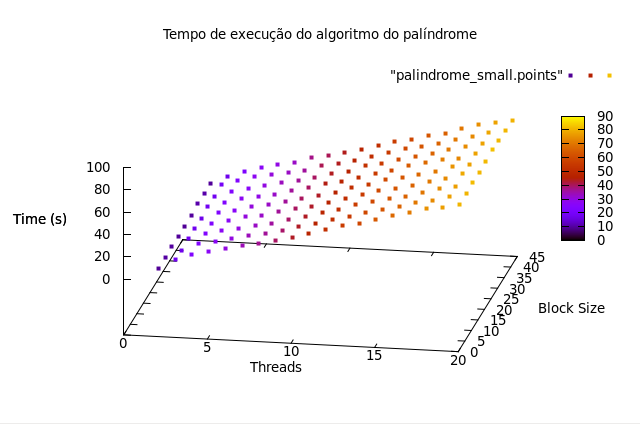
\includegraphics{palindrome-small}}
	\end{center}
	\caption{Resultados do algoritmo do palíndromo para o arquivo menor}
	\label{palindrome-small}
\end{figure}
\begin{figure}[float=h]
	\begin{center}
		\scalebox{0.5}{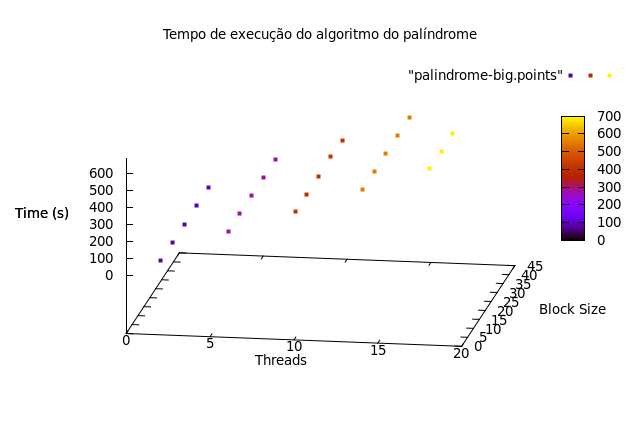
\includegraphics{palindrome-big}}
	\end{center}
	\caption{Resultados do algoritmo do palíndromo para o arquivo maior}
	\label{palindrome-big}
\end{figure}

Os valores do números de threads e o tamanho do bloco que cada thread executará foram baseados em valores estimados. Um cálculo do tamanho médio das palavras provenientes da leitura cega apontou que para o arquivo menor, essa média valia 40 e para o maior, 4.

\newpage
\section{Referências}

\end{document}
